\section{Verbesserung der Abbruchbedingung und -logik}
Die Analyse der Testergebnisse hat gezeigt, dass die Prominenzwerte teilweise fehlerhaft sind. Die Ursache liegt in einer nicht optimal implementierten Abbruchbedingung bei der Prominenzberechnung.

Die bisherige Implementierung ermittelt den Sattelpunkt zum nächstgelegenen höheren Gipfel. Dies entspricht jedoch nicht der korrekten Definition der Prominenz. Die Prominenz (auch Schartentiefe genannt) ist der Höhenunterschied zwischen einem Gipfel und dem höchstgelegenen Sattel, der ihn mit einem höheren Gipfel verbindet \todo{ref def Prominenz}. Dieser Sattel gehört nicht zwangsläufig zum nächstgelegenen höheren Gipfel.

Das Beispiel des Zugspitzecks verdeutlicht dieses Problem (siehe Abbildung \ref{fig:Satelitenbild_Zugspitzeck}). Das Zugspitzeck liegt näher am Schneefernerkopf als an der Zugspitze. Der Sattel zum Schneefernerkopf liegt auf 2699\,m, während der Sattel zur Zugspitze auf 2788\,m liegt. Der Sattel zur Zugspitze ist also der Sattelpunkt. Die alte Implementierung würde fälschlicherweise den Sattel zum näheren Schneefernerkopf wählen und eine Prominenz von 116\,m berechnen, obwohl der korrekte Wert, basierend auf dem Sattel zur Zugspitze, nur 27\,m beträgt.

\begin{figure}[h]
    \centering
    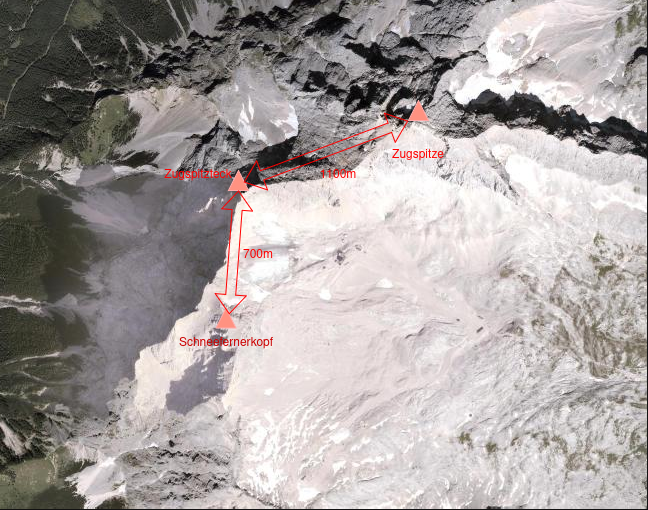
\includegraphics[width=1.0\textwidth]{Diagramms/Abstände_Zugspitzeck.drawio.png}
    \caption{Satelitenbild des Zugspitzecks}
    \label{fig:Satelitenbild_Zugspitzeck}
\end{figure}

Um diesen Fehler zu beheben, wird die Abbruchlogik angepasst. Die neue Abbruchbedingung beendet die Suche, sobald ein Punkt erreicht wird, der höher ist als der Ausgangsgipfel. 

Dieser Ansatz hat zwei Vorteile. Erstens garantiert er das Finden des korrekten, höchsten Sattelpunktes. Da der Suchalgorithmus von einem Pixel immer zum höchstgelegenen Nachbarpixel fortschreitet (ähnlich einer Gradientenabstiegsmethode auf einem Inversrelief), folgt er dem Pfad des geringsten Höhenverlusts. Dieser Pfad führt zwangsläufig über den höchsten Sattel, bevor ein höherer Punkt erreicht wird. Zweitens wird die Berechnungseffizienz gesteigert, da die Suche abgebrochen werden kann, ohne den zugehörigen höheren Gipfel explizit finden zu müssen. Dies reduziert die Anzahl der zu untersuchenden Pixel erheblich.